\documentclass[11pt]{exam}
\usepackage[margin=1in]{geometry}
\pagestyle{plain}
\usepackage{amsmath,amsfonts,amssymb,amsthm,enumerate}
\usepackage{multicol}
\usepackage[]{graphicx}
\usepackage{hyperref}
\usepackage{tikz}
\usepackage{pgfplots}
\usepackage{subfigure}
\usepackage[final]{pdfpages}

\addtolength{\footskip}{2\baselineskip} % to lower the page numbers
\title{\vspace{-0.75in} Math 115 \\ Worksheet Section 2.2}
\date{}


% \theoremstyle{definition}
% \newtheorem{problem}{Problem}
\renewcommand{\questionlabel}{\textbf{Problem~\thequestion.}}
%\printanswers

\begin{document}
\maketitle
\vspace{-0.75in}
\begin{questions}
\question
  \begin{parts}
  \part What is the definition of the derivative of the function
    \(f(x)\) at \(x=c\)?
    \vspace{0.3in}
  \part Compute the derivative of \(g(x) = 3x^2\) at
    \(x=10\) \textbf{algebraically}. In other words, use algebra to
    find the limit from the definition exactly using limit
    computations we learned from the previous sections.
  \end{parts}
  \begin{solution}
    \begin{enumerate}[(a)]
    \item \[
        f'(c) = \lim_{h \to 0} \frac{f(c+h)-f(c)}{h}
      \]
    \item In the above, we set \(c=10\). We compute
      \begin{align*}
        f'(10)
        & = \lim_{h \to 0} \frac{f(10+h)-f(10)}{h} \\
        & = \lim_{h \to 0} \frac{3(10+h)^2-3(10)^2}{h}\\
        & = \lim_{h \to 0} \frac{300+60h+3h^2-300}{h}\\
        & = \lim_{h \to 0} \frac{(60+3h)h}{h}\\
        & = \lim_{h \to 0} 60+3h\\
        & = 60
      \end{align*}
    \end{enumerate}
  \end{solution}
\question (Winter 2018 Exam 1)
Let $m(x) = (1+x^2)^{3x-4}$. Which of the limits below represents
$m'(2)$? There is only one correct answer. Be sure to explain your reasoning on
the board.
\begin{multicols}{2}
\begin{enumerate}[(a)]
\item $\displaystyle\lim_{h \rightarrow 0} \frac{(1+x^2)^{3x-4} + h - 25}{h}$
\item $\displaystyle\lim_{h \rightarrow 0} \frac{(1+h^2)^{3h-4}- 25}{h}$
\item $\displaystyle\lim_{h \rightarrow 0} \frac{(1+(2+h)^2)^{3h-4}- 25}{h}$
\item $\displaystyle\lim_{h \rightarrow 0} \frac{(1+(2+h)^2)^{3h+2}- 25}{h}$
\item $\displaystyle\lim_{h \rightarrow 0} \frac{(5+h^2)^{3h+2}- 25}{h}$
\item $\displaystyle\lim_{h \rightarrow 0} \frac{(1+h^2)^{3h+2}- 25}{h}$
\end{enumerate}
\end{multicols}
\begin{solution}
  We compute that \(m(2+h) = (1+(2+h)^2)^{3(2+h)-4} =
  (1+(2+h)^2)^{3h+2})\) and \(m(2)=(1+2^2)^{2} = 25\). Thus, putting
  the pieces together, the correct answer must be (d).
\end{solution}
\question (2.2 \#27) Create a table using difference quotients to
  approximate the derivative of $x^x$ at $x=2$ to one decimal
  place. You may use a calculator for this problem.
  \begin{solution}
    We want to check values of \[
      \frac{(2+h)^{2+h}-2^2}{h}
    \]
    for values near \(0\). We compute\\
    \begin{tabular}{|r|l|}
      \hline \(h\) & \(\frac{(2+h)^{2+h}-4}{h}\)\\
      \hline 0.1 & 7.5 \\
      \hline 0.01 & 6.8\\
      \hline 0.001 & 6.8\\
      \hline -0.001 & 6.8\\
      \hline -0.01 & 6.7\\
      \hline -0.1 & 6.1\\
      \hline
    \end{tabular}\\
    Thus, we estimate that the derivative of \(x^x\) at \(x=2\) is
    approximately \(6.8\).
  \end{solution}
\question  (2.2 \#11)  Match the derivatives in the table with the points $a,b,c,d,e$.\\
	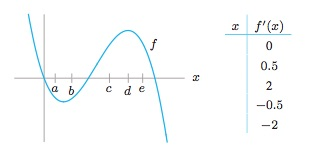
\includegraphics[width=4in]{Figures/no11.jpg}
         \begin{solution}
           \begin{tabular}{|r|l|}
             \hline
             d & 0\\
             \hline 
             b & 0.5\\
             \hline
             c & 2\\
             \hline
             a & -0.5\\
             \hline
             e & -2\\
             \hline
           \end{tabular}
         \end{solution}
\question (2.2 \# 15) For each of the following pairs, use the graph to decide which is larger.  Explain.\\
%	\begin{multicols}{2}
  \begin{minipage}{0.5\linewidth}
    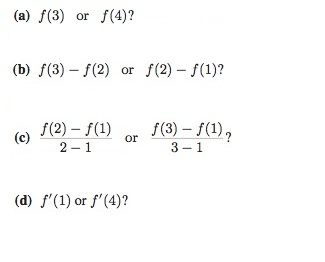
\includegraphics[width=3.2in]{Figures/no15.jpg}
  \end{minipage}
  \begin{minipage}{0.5\linewidth}
    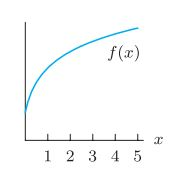
\includegraphics[width=2in]{Figures/no15graph.jpg}
  \end{minipage}
%	 \end{multicols}
         \begin{solution}
           \begin{enumerate}[(a)]
           \item \(f(4)\). It has the higher \(y\)-value.
           \item \(f(2)-f(1)\). The rate of change is gradually
             decreasing, so the difference between \(f(2)\) and
             \(f(1)\) is larger than the difference between \(f(3)\)
             and \(f(2)\).
           \item \(\frac{f(2)-f(1)}{2-1}\). The secant line from
             \((1,f(1))\) to \((2,f(2))\) has larger slope than the
             one from \((1,f(1))\) to \((3,f(3))\).
           \item \(f'(1)\). The slope of the tangent line at \(x=1\)
             is larger than the tangent line at \(x=4\).
           \end{enumerate}
         \end{solution}
\question (2.2 \#17) The given function $f$ has $f(4)=25$ and $f'(4)=1.5$.  Find the coordinates of the points $A, B, C$.
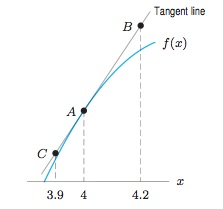
\includegraphics[width=2.5in]{Figures/no17graph.jpg}
\begin{solution}
  Point \(A\) is at \((4,f(4)) = (4,25)\). The tangent line has slope
  \(f'(4) = 1.5\), and \(B\) and \(C\) lie on the tangent line, so we
  get \[
    B = (4.2,25+1.5\cdot(4.2-4)) = (4.2,25+0.3) = (4.2,25.3)
  \]
  and \[
    C = (3.9,25-1.5\cdot(3.9-4)) = (3.9,25-0.15) = (3.9, 24.85)
  \]
\end{solution}
\question (Winter 2016 Exam 1)
Consider the function $g$ defined by
$$g(x) = \left\lbrace\begin{array}{ll} \frac{1}{e^x-1} & \textrm{if } x<\frac{1}{2} \\ \cos(x^x) & \textrm{if } \frac{1}{2} \leqslant x < 5 \\ \frac{x^2}{(x-1)(6-x)} & \textrm{if } x \geqslant 5\end{array}\right.$$
\begin{enumerate}[(a)]
\item Use the limit definition of the derivative to write an explicit expression for $g'(3)$. Your answer should not involve the letter $g$. Do not attempt to evaluate or simplify the limit.
\item Find all vertical asymptotes of $g$, if there are any.
\end{enumerate}
\begin{solution}
  \begin{enumerate}[(a)]
  \item We compute
    \begin{align*}
      g'(3)
      & = \lim_{h \to 0}  \frac{g(3+h)-g(3)}{h} \\
      & = \lim_{h \to 0} \frac{\cos((3+h)^{3+h})-\cos(3^3)}{h}\\
      & = \lim_{h \to 0} \frac{\cos((3+h)^{3+h})-\cos(27)}{h}
    \end{align*}
  \item We check that \(\frac{1}{e^x-1}\) can have a vertical
    asymptote when \(e^x-1 = 0\). This happens when \(e^x = 1\), which
    is when \(x=0\). \(\cos(x^x)\) has no vertical asymptotes for
    \(\frac{1}{2} \leq x < 5\). Finally, \(\frac{x^2}{(x-1)(6-x)}\)
    can have vertical asymptotes at \(x=1\) and \(x=6\) since the
    numerator is non-zero for both inputs but the denominator is
    \(0\). However, we only need to consider the values satisfying \(x
    \geq 5\) for this part of the function. \\

    Thus, \(g(x)\) has vertical asymptotes on \(x=0\) and \(x=6\).
  \end{enumerate}
\end{solution}
\vspace{1in}
\question (Winter 2018 Exam 1) 
Sketch the graph of a single function $y = f(x)$ satisfying all of the following conditions:
\begin{itemize}
\item The domain of $f(x)$ is the interval $-8< x \leqslant 6$.
\item $f(x)$ is continuous on the interval $-8< x <-2$.
\item $f'(-7)=0$.
\item $f(x)$ is decreasing and concave up for all x in the interval $-6 < x < -4$.
\item The average rate of change of $f(x)$ is equal to $0.5$ between $x=-5$ and $x=-2$.
\item $f(0)=2$ and $f'(0) = -1$.
\item $\displaystyle\lim_{x \rightarrow 2^-}  f(x) = f(2)$ and $\displaystyle\lim_{x \rightarrow 2^+}  f(x) < \displaystyle\lim_{x \rightarrow 2^-}  f(x)$.
\item $f(x)$ has constant rate of change on the interval $3 \leqslant x \leqslant 6$.
\end{itemize}
Make sure that your graph is large and unambiguous.
\begin{solution}
  \href{https://dhsp.math.lsa.umich.edu/exams/115exam1/w17/s8.pdf}{https://dhsp.math.lsa.umich.edu/exams/115exam1/w17/s8.pdf}
\end{solution}
\end{questions}
\end{document}
%%% Local Variables:
%%% mode: latex
%%% TeX-master: t
%%% End:
